\chapter{Hello World!}

\section{Hello World!}

\subsection{编程语言(Programming Language)}

程序是为了让计算机去解决某些问题,它由一系列指令构成。但是计算机并不能理解人类的语言,即使是最简单的,例如“计算一下1+2是多少”。\\

计算机采用的是二进制(binary),也就是只能够理解0和1,因此编程语言用于作为人类与计算机之间沟通的桥梁。

\begin{figure}[H]
	\centering
	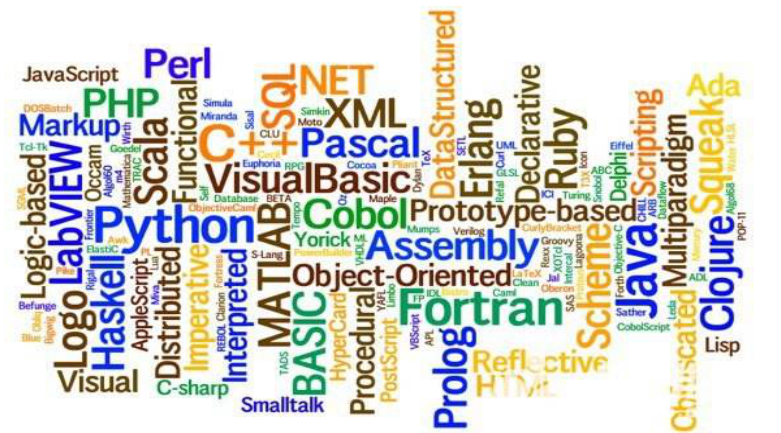
\includegraphics[scale=0.9]{img/Chapter1/1-1/1.png}
\end{figure}

通过使用编程语言来描述解决问题的步骤,从而让计算机一步一步去执行。流程图(flow chat)成为了一种程序的图形化表示方式。\\

\begin{figure}[H]
	\centering
	\begin{tikzpicture}[node distance=2cm]
		\node (start) [startend] {Start};
		\node (init) [io, below of=start] {$ i = 0 $, $ sum = 0 $};
		\node (decision)  [decision, below of=init] {$ i \le 100 $?};
		\node (accumulation) [process, below of=decision] {$ sum = sum + i $};
		\node (update) [process, below of=accumulation] {$ i = i + 1 $};
		\node (output) [io, right of=decision, xshift=2.5cm] {print $ sum $};
		\node (end) [startend, below of=update] {End};

		\draw [arrow] (start) -- (init);
		\draw [arrow] (init) -- (decision);
		\draw [arrow] (decision) -- node[anchor=east] {yes } (accumulation);
		\draw [arrow] (accumulation) -- (update);
		\draw [arrow] (update) -- (-3,-8) -- (-3,-4) -- (decision);
		\draw [arrow] (decision) -- node[anchor=south] {no} (output);
		\draw [arrow] (output) |- (end);
	\end{tikzpicture}
	\caption{计算$ \sum_{i=1}^{100} i $的流程图}
\end{figure}

\vspace{0.5cm}

\subsection{Hello World!}

Hello World是学习编程的第一个程序,它的作用是向屏幕输出"Hello World!"。\\

\mybox{Hello World!}

\begin{lstlisting}[language=C]
#include <stdio.h>

int main()
{
	printf("Hello World!\n");
	return 0;
}
\end{lstlisting}

\begin{tcolorbox}
	\mybox{运行结果}
	\begin{verbatim}
Hello World!
	\end{verbatim}
\end{tcolorbox}

\#include <stdio.h>用于包含标准输入输出库(standard input/output library)的头文件(header file),这样才能够在程序中进行输入输出相关的操作。\\

main()是程序的入口,程序运行后会首先执行main()中的代码。printf()的功能是在屏幕上输出一个字符串(string),其中$ \backslash $n表示输出一个换行符。最后的分号用于表示一条语句的结束,注意不要使用中文的分号。\\

return 0表示main()运行结束,返回值为0,一般返回0用于表示程序正常结束。\\

不同编程语言的Hello World写法大同小异,可以看出编程语言的基本结构是相似的。\\

\mybox{C++}

\begin{lstlisting}[language=C++]
#include <iostream>

using namespace std;

int main() {
	cout << "Hello World!" << endl;
	return 0;
}
\end{lstlisting}

\vspace{0.5cm}

\mybox{Java}

\begin{lstlisting}[language=Java]
public class HelloWorld {
    public static void main(String[] args) {
        System.out.println("Hello World!");
    }
}
\end{lstlisting}

\vspace{0.5cm}

\mybox{Python}

\begin{lstlisting}[language=Python]
print("Hello World!")
\end{lstlisting}

\vspace{0.5cm}

\subsection{注释(Comment)}

注释就是对代码的解释和说明,它并不会程序所执行。注释能提高程序的可读性,让人更加容易了解代码的功能。\\

注释一般分为单行注释和多行注释:

\begin{enumerate}
	\item 单行注释:以//开头,该行之后的内容视为注释。
	\item 多行注释:以/*开头,*/结束,中间的内容视为注释。
\end{enumerate}

\vspace{0.5cm}

\mybox{注释}

\begin{lstlisting}[language=C]
/*
* Author: Terry
* Date: 2022/11/16
*/

#include <stdio.h>      // header file

int main()
{
	printf("Hello World!\n");
	return 0;
}
\end{lstlisting}

\newpage

\section{数据类型}

\subsection{数据类型(Data Types)}

在计算机中,每个数据一般都有一个对应的类型,基础数据类型包括:

\begin{enumerate}
	\item 整型
	      \begin{itemize}
		      \item 短整型short
		      \item 整型int
		      \item 长整型long
		      \item 长长整型long long
	      \end{itemize}

	\item 浮点型
	      \begin{itemize}
		      \item 单精度浮点数float
		      \item 双精度浮点数double
	      \end{itemize}

	\item 字符型char
\end{enumerate}

\vspace{0.5cm}

不同的数据类型所占的内存空间大小不同,因此所能表示的数值范围也不同。\\

\begin{table}[H]
	\centering
	\setlength{\tabcolsep}{5mm}{
		\begin{tabular}{|c|c|c|}
			\hline
			\textbf{数据类型} & \textbf{大小} & \textbf{取值范围}                                 \\
			\hline
			short             & 2字节         & $ -2^{15} \sim 2^{15} - 1 $                       \\
			\hline
			int               & 4字节         & $ -2^{31} \sim 2^{31} - 1 $                       \\
			\hline
			long              & 4字节         & $ -2^{31} \sim 2^{31} - 1 $                       \\
			\hline
			long long         & 8字节         & $ -2^{63} \sim 2^{63} - 1 $                       \\
			\hline
			float             & 4字节         & $ 1.2 \times 10^{-38} \sim 3.4 \times 10^{38} $   \\
			\hline
			double            & 8字节         & $ 2.3 \times 10^{-308} \sim 1.7 \times 10^{308} $ \\
			\hline
			char              & 1字节         & $ -128 \sim 127 $                                 \\
			\hline
		\end{tabular}
	}
\end{table}

\vspace{0.5cm}

\subsection{变量(Variable)}

变量是用来存储数据的内存空间,每个变量都有一个类型,变量中只能存储对应类型的数据。

\vspace{-0.5cm}

\begin{lstlisting}[language=C]
int num = 10;
double wage = 8232.56;
\end{lstlisting}

\vspace{0.5cm}

变量的命名需要符合规范:

\begin{enumerate}
	\item 由字母、数字和下划线组成,不能以数字开头
	\item 不可以使用编程语言中预留的关键字
	\item 使用英语单词,顾名思义
\end{enumerate}

关键字是编程语言内置的一些名称,具有特殊的用处和意义,因此不应该作为变量名,防止产生歧义。\\

\begin{table}[H]
	\centering
	\setlength{\tabcolsep}{5mm}{
		\begin{tabular}{|c|c|c|c|c|}
			\hline
			auto     & break   & case   & char     & const  \\
			\hline
			continue & default & do     & double   & else   \\
			\hline
			enum     & extern  & float  & for      & goto   \\
			\hline
			if       & int     & long   & register & return \\
			\hline
			short    & signed  & sizeof & static   & struct \\
			\hline
			switch   & typedef & union  & unsigned & void   \\
			\hline
			volatile & while   & inline & restrict &        \\
			\hline
		\end{tabular}
	}
	\caption{关键字}
\end{table}

\vspace{0.5cm}

\subsection{常量(Constant)}

变量的值在程序运行过程中可以修改,但有一些数据的值是固定的,为了防止这些数据被随意改动,可以将这些数据定义为常量。\\

在数据类型前加上const关键字,即可定义常量,常量一般使用大写表示。如果在程序中尝试修改常量,将会报错。\\

\mybox{常量}

\begin{lstlisting}[language=C]
#include <stdio.h>

int main()
{
	const double PI = 3.1415;
	PI = 4;
	return 0;
}
\end{lstlisting}

\begin{tcolorbox}
	\mybox{运行结果}\\
	\textcolor{red}{error: assignment of read-only variable "PI"}
\end{tcolorbox}

\newpage

\section{输入输出函数}

\subsection{printf()}

printf()的功能是向屏幕输出指定格式的文本,但是有些需要输出的字符在编程语言中具有特殊含义,因此这些特殊的字符,需要经过转义后输出。\\

\begin{table}[H]
	\centering
	\setlength{\tabcolsep}{5mm}{
		\begin{tabular}{|c|c|}
			\hline
			\textbf{转义字符}      & \textbf{描述}                \\
			\hline
			\lstinline|\\| & 反斜杠\lstinline|\| \\
			\hline
			\lstinline|\'| & 单引号\lstinline|'| \\
			\hline
			\lstinline|\"| & 双引号\lstinline|"| \\
			\hline
			\lstinline|\n| & 换行                         \\
			\hline
			\lstinline|\t| & 制表符                       \\
			\hline
		\end{tabular}
	}
	\caption{转义字符}
\end{table}

\mybox{转义字符}

\begin{lstlisting}[language=C]
#include <stdio.h>

int main()
{
	printf("\"Hello\nWorld\"");
	return 0;
}
\end{lstlisting}

\begin{tcolorbox}
	\mybox{运行结果}
	\begin{verbatim}
"Hello
World"
	\end{verbatim}
\end{tcolorbox}

在对变量的值进行输出时,需要在printf()中使用对应类型的占位符。\\

\begin{table}[H]
	\centering
	\setlength{\tabcolsep}{5mm}{
		\begin{tabular}{|c|c|}
			\hline
			\textbf{数据类型} & \textbf{占位符} \\
			\hline
			int               & \%d             \\
			\hline
			float             & \%f             \\
			\hline
			double            & \%f             \\
			\hline
			char              & \%c             \\
			\hline
		\end{tabular}
	}
	\caption{占位符}
\end{table}

\vspace{0.5cm}

\mybox{长方形面积}

\begin{lstlisting}[language=C]
#include <stdio.h>

int main()
{
	int length = 10;
	int width = 5;
	double area;

	area = length * width;
	printf("Area = %d * %d = %.2f\n", length, width, area);
	return 0;
}
\end{lstlisting}

\begin{tcolorbox}
	\mybox{运行结果}
	\begin{verbatim}
Area = 10 * 5 = 50.00
	\end{verbatim}
\end{tcolorbox}

\vspace{0.5cm}

\subsection{scanf()}

有时候一些数据需要从键盘输入,scanf()可以读取对应类型的数据,并赋值给相应的变量。\\

在被赋值的变量前需要使用取地址符\&,因为scanf()需要将读取到的数据保存到该变量的内存地址中。\\

在使用scanf(),通常会使用printf()先输出一句提示信息,告诉用户需要输入什么数据。\\

\mybox{圆面积}

\begin{lstlisting}[language=C]
#include <stdio.h>
#include <math.h>

int main()
{
	const double PI = 3.14159;
	double r;
	double area;

	printf("Radius: ");
	scanf("%lf", &r);

	area = PI * pow(r, 2);
	printf("Area = %.2f\n", area);
	return 0;
}
\end{lstlisting}

\begin{tcolorbox}
	\mybox{运行结果}
	\begin{verbatim}
Radius: 5
Area = 78.54
	\end{verbatim}
\end{tcolorbox}

头文件math.h中定义了一些常用的数学函数,例如pow(x, y)可用于计算$ x $的$ y $次方。\\

\newpage

\section{表达式}

\subsection{算术运算符}

大部分编程语言中的除法与数学中的除法意义不同。\\

当相除的两个数都为整数时,那么就会进行整除运算,因此结果仍为整数,例如21 / 4 = 5。\\

如果相除的两个数中至少有一个为浮点数时,那么就会进行普通的除法运算,结果为浮点数,例如21.0 / 4 = 5.25。\\

取模(modulo)运算符\%用于计算两个整数相除之后的余数,例如22 \% 3 = 1、4 \% 7 = 4。\\

\mybox{逆序三位数}

\begin{lstlisting}[language=C]
#include <stdio.h>

int main()
{
	int num;
	int a, b, c;

	printf("Enter a 3-digit integer: ");
	scanf("%d", &num);

	a = num / 100;
	b = num / 10 % 10;
	c = num % 10;

	printf("Reversed: %d\n", c*100 + b*10 + a);
	return 0;
}
\end{lstlisting}

\begin{tcolorbox}
	\mybox{运行结果}
	\begin{verbatim}
Enter a 3-digit integer: 520
Reversed: 25
	\end{verbatim}
\end{tcolorbox}

\vspace{0.5cm}

\subsection{复合运算符}

使用复合运算符可以使表达式更加简洁。例如\lstinline|a = a + b|可以写成\lstinline|a += b|,-=、*=、/=、\%=等复合运算符的使用方式同理。\\

当需要给一个变量的值加/减1时,除了可以使用\lstinline|a += 1|或\lstinline|a -= 1|之外,还可以使用++或--运算符,但是\lstinline|++|和\lstinline|--|可以出现在变量之前或之后:\\

\begin{table}[H]
	\centering
	\setlength{\tabcolsep}{5mm}{
		\begin{tabular}{|c|l|}
			\hline
			\textbf{表达式}         & \textbf{含义}         \\
			\hline
			\lstinline|a++| & 执行完所在语句后自增1 \\
			\hline
			\lstinline|++a| & 在执行所在语句前自增1 \\
			\hline
			\lstinline|a--| & 执行完所在语句后自减1 \\
			\hline
			\lstinline|--a| & 在执行所在语句前自减1 \\
			\hline
		\end{tabular}
	}
	\caption{自增/自减运算符}
\end{table}

\mybox{自增/自减运算符}

\begin{lstlisting}[language=C]
#include <stdio.h>

int main()
{
	int n = 10;

	printf("%d\n", n++);
	printf("%d\n", ++n);
	printf("%d\n", n--);
	printf("%d\n", --n);

	return 0;
}
\end{lstlisting}

\begin{tcolorbox}
	\mybox{运行结果}
	\begin{verbatim}
10
12
12
10
	\end{verbatim}
\end{tcolorbox}

\vspace{0.5cm}

\subsection{隐式类型转换}

在计算机计算的过程中,只有类型相同的数据才可以进行运算。例如整数+整数、浮点数/浮点数等。\\

但是很多时候,我们仍然可以对不同类型的数据进行运算,而并不会产生错误,例如整数+浮点数。这是由于编译器会自动进行类型转换。在整数+浮点数的例子中,编译器会将整数转换为浮点数,这样就可以进行运算了。\\

编译器选择将整数转换为浮点数,而不是将浮点数转换为整数的原因在于,浮点数相比整数能够表示的范围更大。例如整数8可以使用8.0表示,而浮点数9.28变为整数9后就会丢失精度。\\

隐式类型转换最常见的情形就是除法运算,这也是导致整数/整数=整数、整数/浮点数=浮点数的原因。\\

\subsection{显式类型转换}

有些时候编译器无法自动进行类型转换,这时就需要我们手动地强制类型转换。\\

\mybox{显式类型转换}

\begin{lstlisting}[language=C]
#include <stdio.h>

int main()
{
	int total = 821;
	int num = 10;
	double average = (double)total / num;
	printf("Average = %.2f\n", average);
	return 0;
}
\end{lstlisting}

\begin{tcolorbox}
	\mybox{运行结果}
	\begin{verbatim}
Average = 82.10
	\end{verbatim}
\end{tcolorbox}

\newpage